\section{Requirements-Engineering}\label{section:Requirements-Engineering}

Um ein vollständiges Konzept über das zu entwickelnde regelbasiertes Validationssystem (\textit{ARVal}), soll zunächst ein strukturiertes Requirements-Engineering nach \textcite{ieeeISOIECIEEE2018} und \textcite{ruppRequirementsEngineeringUndManagement2021} durchgeführt werden.

Durch die ausführliche Anforderungserhebung des Systems sollen alle Aspekte vollständig berücksichtigt, argumentiert und kontextualisiert werden, bevor die Implementierung durchgeführt wird. Hierdurch soll sichergestellt werden, dass das entwickelte System schlüssig und logisch begründet, sowie nachvollziehbar ist.

\subsection{Projektkontext und Scope}\label{subsection:Projektkontext und Scope}

Das Ziel des Projekts ist die Implementierung eines browser-basierten Moduls zur Echtzeit-Validierung von platzierten AR-Objekten, basierend auf einem definierten Constraint-Set.

Abgegrenzt hierzu ist die Implementierung des Basisprojekts zur Darstellung der AR-Elemente, Integration von Gerätedaten und Untersuchung von Basistechnologien. Diese Aspekte wurden bereits in den vorangegangenen Forschungsprojekten untersucht. Die Ergebnisse dieser Projekte werden während der Implementierung für diese Arbeit aufgearbeitet, für das Requirements Engineering werden diese daher jedoch nicht behandelt.

\subsubsection{Projektbegriffe}

Für die Argumentation des Systems werden zunächst die genutzten Begriffe genauer definiert und eingeschränkt:

\begin{enumerate}
    \item \textbf{Validierungssystem}: Das Validierungssystem beschreibt die zu entwickelnde Software-Komponente, die Objektdaten entgegennimmt, Regeln prüft und ein Ergebnis (\textmono{valid}, \textmono{violations[]}) liefert.
    \item \textbf{AR-Basissystem}: Das Basissystem bezeichnet die Client-Webseite, in der Bürger:innen Objekte platzieren und Visualisierungen sehen. Diese wurde bereits in den vorangegangenen Forschungsprojekten aufgestellt und wird für diese Arbeit als Startpunkt genutzt.
    \item \textbf{Regelpaket}: Als Regelpaket wird die Definition aller Regeln eines Objekttyps bezeichnet. Für jedes Objekt sollen dabei zukünftig alle Regeln im Regelpaket validiert werden.
\end{enumerate}

\subsubsection{Projektziel und Nutzen}

Das Ziel des Projekts (\textit{Business Goals} bzw. \textit{Mission Needs}) ist die Verbesserung der Qualität von Bürgervorschlägen durch frühzeitige Validierung, die Reduktion des manuellen Prüfaufwands für die Stadtverwaltung, eine Erhöhung der Akzeptanz und des Verständnisses für stadtplanerische Einschränkungen bei Bürger:innen sowie die Schaffung einer effizienten Schnittstelle zwischen Bürger-Input und stadtplanerischen Regelwerken.

Der daraus resultierende Nutzen für Bürger:innen besteht im sofortigen Feedback, höhere Erfolgswahrscheinlichkeit ihrer Vorschläge sowie ein besseres Verständnis für Planungsrestriktionen. Für Stadtplaner:innen und Verwaltungen besteht der Nutzen des Systems in qualitativ hochwertigeren Vorschlägen, weniger fehlerhaften Einreichungen und einer effizienteren Prüfung.

\subsubsection{Abgrenzung}

\begin{table}[!h]
\begin{center}
\bgroup
\def\arraystretch{1.5}
    \begin{tabular}{| p{7cm} | p{7cm} |}
    \hline
    In Scope (MVP) & Out of Scope \\
    \hline
    \hline
    
    Nutzung der Objektplatzierung und Standortbestimmung vom Basissystem zur Validierung & Routenplanung \\
    \hline
    Regelvalidierung (Constraints) & Tiefbau-Genehmigungen \\
    \hline
    Visuelles Feedback (Grün / Rot) & Budget-Bewertungen \\
    \hline
    Definition einer Constraint-Syntax & Visueller Editor zur Bearbeitung von Constraints \\
    \hline
    Segmentierung der Umgebung zwischen Straßen, Gehwegen und Grünflächen & Segmentierung der Umgebung in weitere Kategorien (z.B. Gebäude, Fahrradständer, existierende Objekte etc.) \\
    \hline
     & Backend zum Upload und Verwaltung, Benutzerverwaltung und Authentifizierung und Persistente Speicherung von Nutzervorschlägen im Validierungssystem \\
     \hline
     & Komplexe Manipulation von Objekten (z.B. eine Bank mit dynamisch anpassbarer Länge) \\
     \hline
    
    \end{tabular}
    \egroup
    
\caption{Projektabgrenzung}
\label{tab:Projektabgrenzung}
\end{center}
\end{table}

Zur Abgrenzung des Projektumfangs enthält Tabelle \ref{tab:Projektabgrenzung} eine Einordnung zwischen In-Scope und Out of Scope Bestandteilen. In-Scope sind insbesondere alle essenziellen Bestandteile zur Validierung, darunter der Constraint-Syntax, Regelvalidierung und Integration in das Basissystem. Explizit Out of Scope sind hierbei alle optionalen Bestandteile, welche nicht direkt für die Validierung von Objekten notwendig sind - darunter etwa die Bewertung des Budgets für Vorschläge sowie ein Backend zum Upload dieser.

\subsection{Elicitation}\label{subsection:Elicitation}

Für eine vollständige, umfassende Aufarbeitung der benötigten Komponenten wurde zunächst eine mehrteilige Erhebung aller relevanten Ressourcen durchgeführt. Hierbei wurden verschiedene Techniken kombiniert, darunter ein Dokumentenstudium, aufgearbeitet in Kapitel \ref{section:Verwandte Arbeiten}, ein Experteninterview, aufgearbeitet in Kapitel \ref{subsubsection:Interview mit Prof. Koch}, sowie Beobachtungstechniken zu bisherigen Technologien, aufgearbeitet in Kapitel \ref{subsubsection:Analyse existierender Constraint-Systeme}.

\subsubsection{Interview mit Prof. Koch}\label{subsubsection:Interview mit Prof. Koch}

Für die Erhebung von Anforderungen aus Sicht der Stadtplanung wurde ein qualitatives, halbstrukturiertes Experteninterview mit Prof. Dr. Florian Koch, Professor für Immobilienwirtschaft, Stadtentwicklung und Smart Cities an der HTW Berlin, durchgeführt \parencite{kochStartseiteProfDr2025}.

TODO
% Interview mit Prof. Koch, Stadtplaner, über häufige Vorschläfe, nötige Einschränkungen etc.

\subsubsection{Analyse existierender Constraint-Systeme}\label{subsubsection:Analyse existierender Constraint-Systeme}

TODO
- Analyse existierender Mängelmeldungs-Apps (Competitive Benchmark).
Untersuchung existierende CAD, Game Design etc.


\subsection{Stakeholder und Nutzungsszenarien}\label{subsection:Stakeholder und Nutzungsszenarien}

Nachfolgend sollen die Stakeholder und häufige Nutzungsszenarien von \textit{ARVal} untersucht werden.

\subsubsection{Nutzergruppen}

\begin{figure}[h]
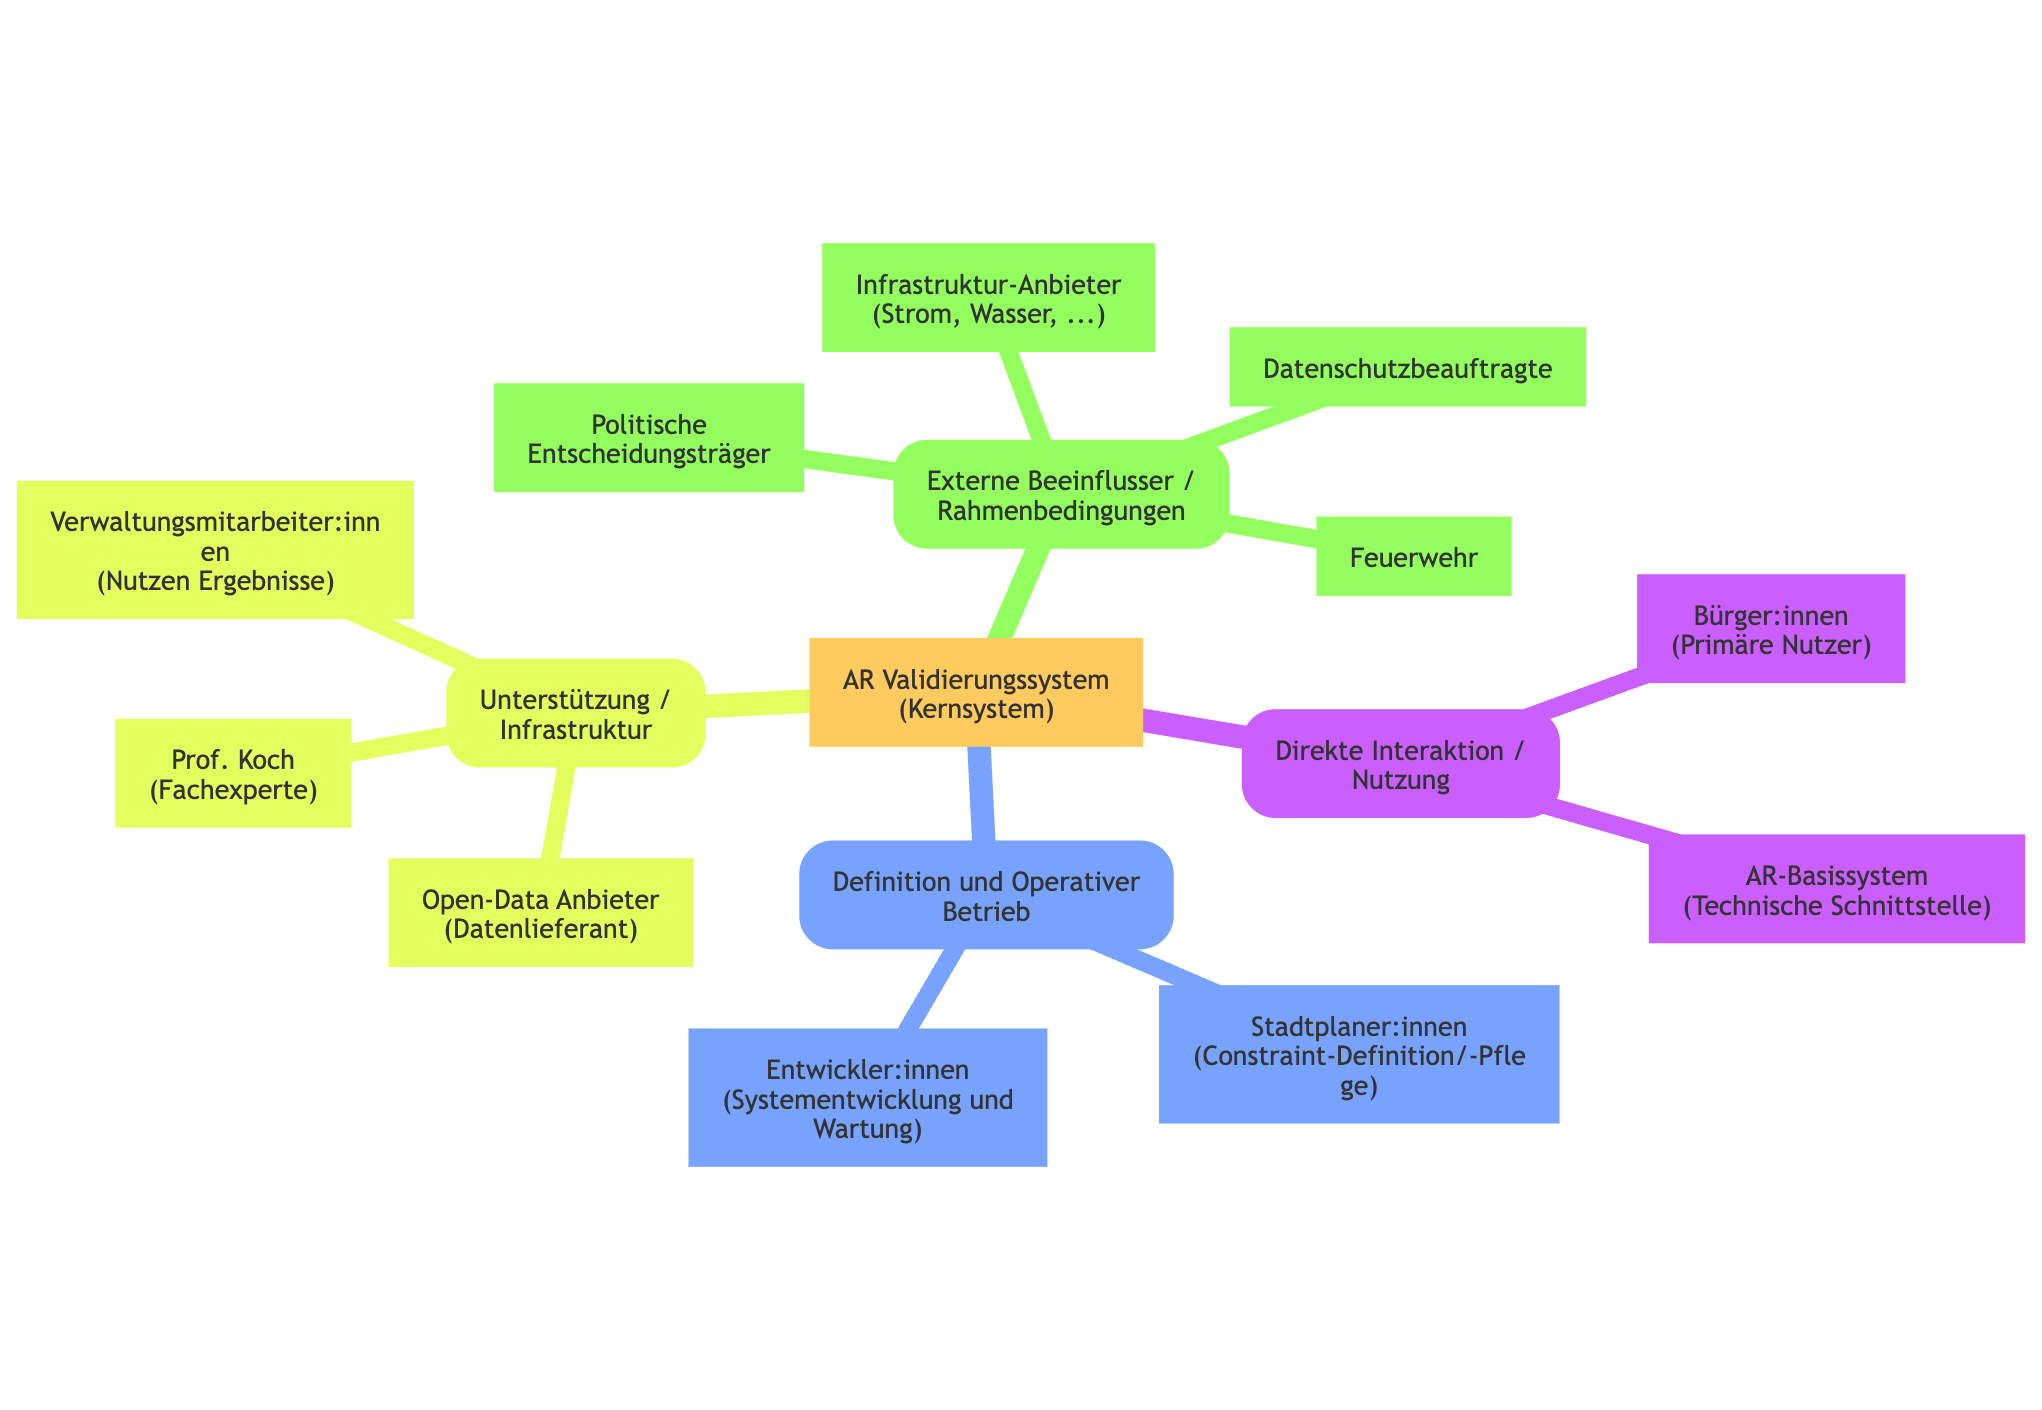
\includegraphics[width=0.9\textwidth]{abb/stakeholder onion model.png}
\centering
\caption{Stakeholder Onion Model (eigene Abbildung)}
\label{fig:Stakeholder Onion Model}
\end{figure}

Abbildung \ref{fig:Stakeholder Onion Model} stellt das entwickelte Onion-Model zur Stakeholderanalyse dar. Im Kern ist hierbei das AR Validierungssystem, von welchem die vier Gruppen der direkten Nutzer, Definition und operativer Betrieb, Unterstützung bzw. Infrastruktur und externe Beeinflusser identifiziert wurden.

Als primäre Nutzergruppe wurden Bürger:innen identifiziert, die das System aktiv zur Validierung ihrer AR-Platzierungen nutzen. Diese Gruppe steht in direktem Kontakt mit den Ausgaben des Systems und nutzen dieses, um die eigenen Vorschläge zu verbessern.

Als sekundäre Nutzergruppe wurden Stadtplaner:innen eruiert, welche die Definition der Constraints über den auszuarbeitenden Constraint-Syntax definieren.

Ebenfalls sekundäre Nutzer, welche der Infrastruktur zugeordnet wurden, sind Verwaltungen, welche von den verbesserten Vorschlägen durch die Validierung profitieren.

Neben diesen Hauptakteuren wurden ebenfalls Rahmenankteure wie Datenschutzbeaufragte für die Verwendung von Standortdaten sowie politische Entscheidungsträger:innen mit Interesse an erfolgreicher Bürgerbeteiligung festgestellt.

In der Gruppe der Enabler wurden schließlich die Entwickler, welche die Erstellung Wartung des Systems durchführen, sowie Open-Data Anbieter wie OpenStreetMap, welche Schnittstellen für genutzte Daten des Validierungssystems liefern, ermittelt.

\medskip

Auf Basis der ermittelten Stakeholder wurde eine Stakeholder-Tabelle mit Hauptinteressen, Erwartungen, Einfluss und potenziellen Konflikten aufgestellt, welche in Tabelle \ref{tab:Stakeholder-Tabelle} [S. \pageref{tab:Stakeholder-Tabelle}, \ref{anh:Stakeholder}] abgebildet ist.

Wichtige potenzielle Konflikte zwischen in den Nutzergruppen sind hierbei der Wunsch nach maximaler Freiheit gegen restriktive Regeln bei Bürger:innen und die unterstützte Komplexität der Regeln für Stadtplaner:innen gegen die Performance und Verständlichkeit für Bürger:innen.

\subsubsection{Nutzungsszenarien}

Aufbauend auf den erarbeiteten Informationen zu Stakeholdern wurden User Stories definiert. Die vollständige Tabelle aller User Stories ist in Tabelle \ref{tab:User Stories} [S. \pageref{tab:User Stories}, \ref{anh:Nutzungsszenarien}] abgebildet. Die Stories wurden hierfür für jede Stakeholdergruppe einzeln definiert und folgen dem Schema „US-\textit{Stakeholdergruppe}-\textit{Nummer}“, z.B. \textit{US-SP-005}, für die spätere Referenzierung.

Zu den User Stories für Bürger:innen zählen hierbei insbesondere solche, die sicherstellen, dass die Validierung schnell und verständlich stattfindet. Hierzu zählen Stories zur Darstellung eines Live-Status bei der Verschiebung und eine Auskunft durch die Hinterlegung des Objekts in roter Farbe.

Für Stadtplaner:innen fokussieren sich die Stories auf die Definition der formalen Constraints sowie bestimmte Arten von Constraints - etwa Einschränkung der Rotation oder Untergründe.

Für Entwickler:innen des Systems liegt der Fokus insbesondere auf die Erstellung eines stabilen, performanten Interfaces.

\medskip

Zur besseren Gruppierung und Überblick zu wichtigen Funktionen wurde anschließend eine Use Case Tabelle ausgearbeitet. Diese ist als Tabelle \ref{tab:Use Cases} [S. \pageref{tab:Use Cases}, \ref{anh:Nutzungsszenarien}] abgebildet. Die einzelnen Use Cases werden zudem in den Tabellen \ref{tab:UC-VAL-001} [S. \pageref{tab:UC-VAL-001}, \ref{anh:Nutzungsszenarien}] bis \ref{tab:UC-DEV-001} [S. \pageref{tab:UC-DEV-001}] genauer untersucht. Die Use Cases referenzieren hierbei jeweils diejenigen User Stories, welche sie zusammenfassen.

Die Use-Cases folgen dem Namensschema „UC-\textit{Bereich}-\textit{Nummer}“, z.B. \textit{UC-VAL-002}. Die Aufteilung geschieht in die Bereiche Validierung (\textit{VAL}), Administration (\textit{ADM}) und Entwicklung (\textit{DEV}).

Für die Validierung aus Sicht von Bürger:innen wurde hierbei als primäre Use Cases definiert, dass die Objektplatzierung validiert werden kann und während der Verschiebung von Objekten eine direkte Rückmeldung erfolgt.

Für die Administration war der primäre Use Case das einfache Definieren und verwalten von Constraints der einzelnen Objekte.

Zuletzt war es für die Entwicklung von hohem Wert, dass die Validierung über ein typisiertes Interface modular konsumiert werden kann.

\subsubsection{Zielmodellierung}

TODO: Goal Model (i* 2.0) zur Ableitung von Constraints als hard goals.

\subsubsection{Szenario-Modellierung}

Viele der Einzelheiten des Systems wurden in den vorherigen Modellen bereits untersucht und definiert. Während der Iteration dieser Modelle wurde zusätzlich eine Modellierung zwei essenzieller Szenarien als Sequenzdiagramm erstellt. Hierdurch konnte das Zusammenspiel der einzelnen Komponenten klarer betrachtet werden und über blinde Flecken zwischen den Schichten iteriert werden.

\begin{figure}[h]
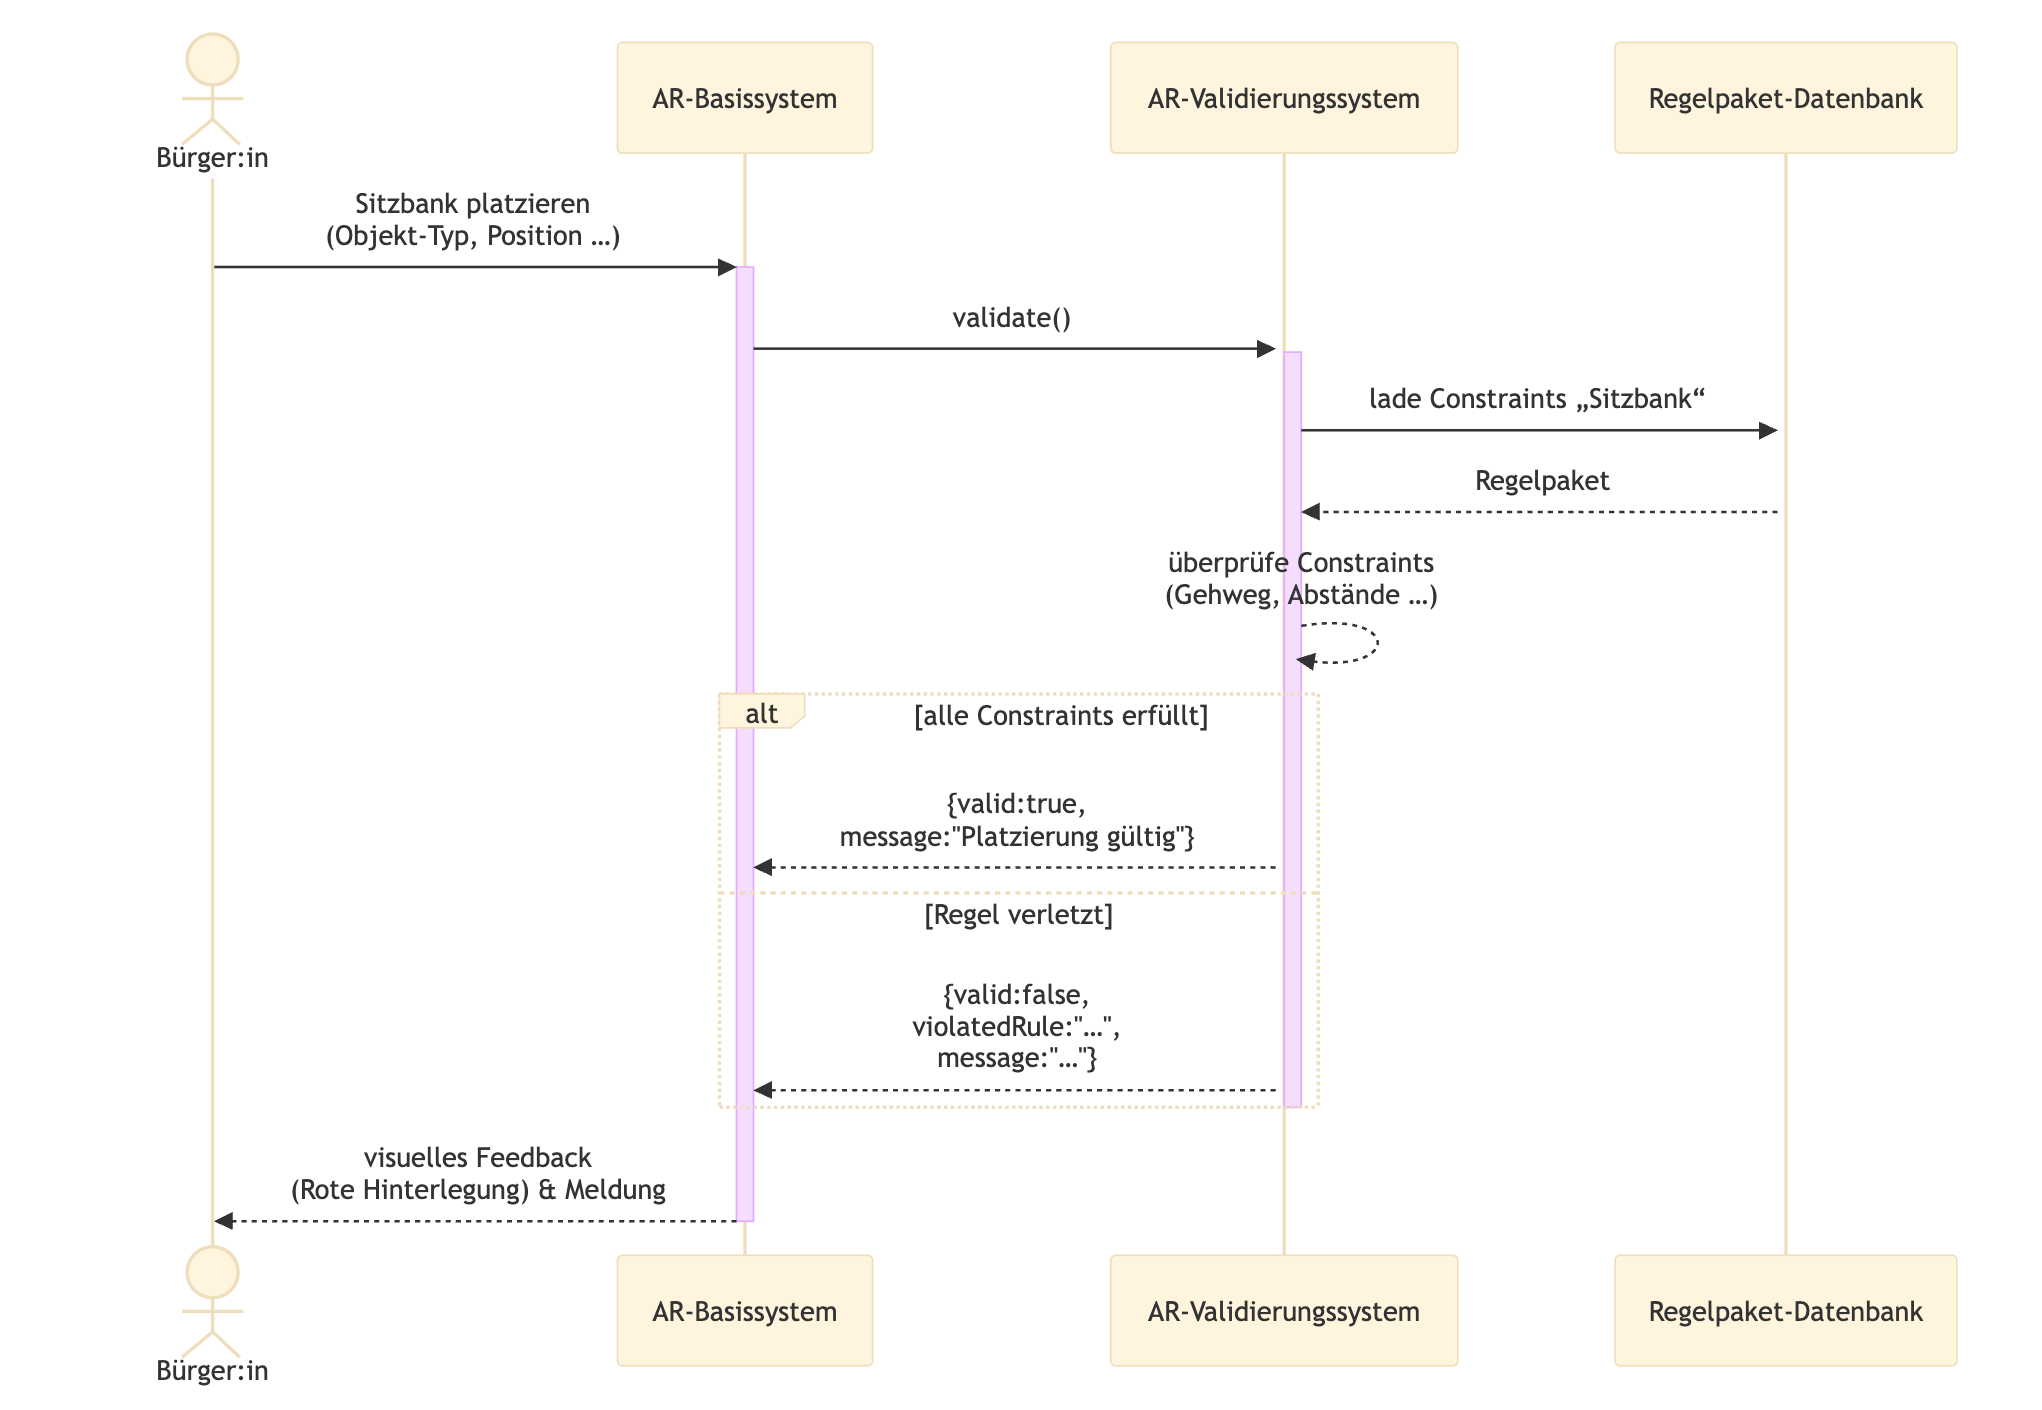
\includegraphics[width=0.9\textwidth]{abb/sequenz_constraint_val.png}
\centering
\caption{Sequenzdiagramm zur Validierung eines Objekts (eigene Abbildung)}
\label{fig:Sequenz Validierung}
\end{figure}

Abbildung \ref{fig:Sequenz Validierung} zeigt das erstellte Sequenzdiagramm zur Validierung einer Objektplatzierung. Die Akteure dieses Diagramms sind der Bürger, welcher das System nutzt, das AR-Basissystem zur AR-Darstellung, das AR-Validierungssystem und die Regelpaket-Datenbank, welche von den Stadtplaner:innen gepflegt wird.

Wenn der Bürger ein Objekt platziert oder verschiebt, ruft das Basissystem das neue Validierungssystem über die Schnittstelle \textmono{validate()} auf. Das Validierungssystem kann sich aus dem Basissystem die Daten über die Objekte und Platzierungen holen, um diese zu validieren.

Das Validierungssystem sollte nun die benötigten Regeln aus der Regelpaket-Datenbank lasen und die enthaltenden Constraints prüfen. Das Ergebnis dieser Prüfung kann schließlich an das Basissystem als valide oder nicht valide  zurückgemeldet werden und per visuellem Feedback dem Bürger dargestellt werden.

TODO: Second Diagram

\subsection{Systemanforderungen}\label{subsection:Systemanforderungen}

Durch die strukturierte, iterative Bearbeitung der Stakeholder, Projektziele und Nutzungsszenarien konnte ein umfangreicher Überblick über das Zielsystem geschaffen werden.

Auf Basis dieser Informationen wurde nachfolgend eine finale Liste an Systemanforderungen erstellt. Die Anforderungen wurden anhand der 17 Regeln des SOPHIST-REgelwerks validiert und iteriert, um eindeutige, umsetzbare Ziele zu definieren \parencite[S. 174-191]{ruppRequirementsEngineeringUndManagement2021}

Die Nummerierung erfolgt hierbei im IEEE-Format als „REQ-\textit{Typ}-\textit{Nummer}“, z.B. \textit{REQ-F-002} für eine funktionale Anforderung. Zusätzlich zu funktionalen (\textit{F}) und nicht-funktionalen (\textit{NF}) Anforderungen, werden zusätzlich Constraint-Anforderungen (\textit{C}) aufgeführt, für die konkreten Constraint-Arten, welche implementiert werden sollen.

\medskip

Die Tabelle aller Systemanforderungen ist als Tabelle \ref{tab:Systemanforderungen} [S. \pageref{tab:Systemanforderungen}, \ref{anh:Systemanforderungen}] zu finden.

Die Anforderungen behandeln die Zusammenarbeit zwischen den verschiedenen Teilsystemen (z.B. REQ-F-001), Einzelheiten zur Schema-Funktionen (z.B. REQ-F-007), Performance-Ansprüche an die Validierung (z.B REQ-NF-001), sowie die konkreten Basisconstraints, welche aus der Elicitation-Phase erarbeitet wurden (z.B. REQ-C-001).

Die Anforderungen enthalten jedoch keine konkreten Implementierungsdetails zum Aussehen des Constraint-Syntax, den inneren Funktionalitäten des Validierungssystems sowie der Segmentierungsmethode. Diese Details sollen in den Kapiteln \ref{section:Konzeptualisierung eines Constraint-Systems} und \ref{section:Implementierung des Constraint-Systems} genauer betrachtet und final aufgearbeitet werden.

\subsubsection{Abgedeckte Objektklassen}

Zur effektiven Prüfung des Validierungssystems soll eine kleine Auswahl von Objekten ermittelt werden, auf welche eine große Breite unterschiedlicher Constraints angewendet werden kann.

Die Fokus liegt hierbei auf einer geringen Auswahl von Objekten mit einer großen Bandbreite von Constraints, anstatt einer großen Bandbreite von Objekten auf die größtenteils die gleichen Constraints angewendet werden müssen.

Auf Basis der Ergebnisse der Elicitation-Phase (Kapitel \ref{subsection:Elicitation}) wurde eine Liste von geeigneten Objekten definiert.

Zunächst wird eine Sitzbank als 3D-Basisobjekt gewählt. Diese bildet ein generisches Beispiel für viele ähnliche Objekte dar, etwa Fahrradständer, Laternen oder Sportfreizeitgeräte. Auf das Objekt können grundlegende Regeln wie eine Platzierung nur auf Grünflächen und eine Rotation nur um die y-Achse angewendet werden, ohne direkt eine zu hohe Spezialisierung zu benötigen. Das Objekt eignet sich daher gut, um als Erstes in das System implementiert zu werden und für die grundlegende Systemvalidierung zu dienen.

Als zweites Element wurde ein Zebrastreifen gewählt. Diese Straßenmarkierung dient als Basisobjekt für ähnliche 2D-Objekte, ohne eine zu hohe Komplexität zu bieten. Das Objekt kann mit einer Standardbreite einer typischen 2-spurigen Straße angelegt werden und geht so nicht in den Out of Scope Bereich der komplexen Objektmanipulation ein. Auch bei diesem Objekt können einige Constraints wie die flache Platzierung und vollständiges Auflegen auf der Straße umgesetzt werden.

Zuletzt können optional als finale Objekte Pflanzenkübel und Bäume hinzugefügt werden. Diese Objektkombination bietet eine interessante Kombination an, bei welcher Bäumen erlaubt werden können, innerhalb von Pflanzenkübeln platziert zu werden. Hierdurch können auch Interaktionen zwischen virtuellen Objekten validiert und umgesetzt werden.

\medskip

Die Objekte sollen in der Umsetzung in der hier genannten Reihenfolge implementiert werden, je nachdem, was für ein Umfang im Rahmen der Arbeit umsetzbar ist. In den drei Iterationen von 3D-Objekten, 2D-Objekten und virtual-virtual Interaktionen können jeweils sehr unterschiedliche Funktionen hinzugefügt und validiert werden.

\subsubsection{Klassifizierung der Constraints}

TODO
z.B. Räumliche Constraints, Semantische Constraints, Interaktive Constraints

\subsection{Priorisierung und Rückverfolgbarkeit}\label{subsection:Priorisierung und Rückverfolgbarkeit}

MoSCoW

\subsection{Qualitätssicherung}\label{subsection:Qualitätssicherung}

Die Anforderungen wurden nach dem SOPHIST-REgelwerk geprüft